\section{Problem 2}
\subsection{Technics}

    \begin{frame}[fragile]
        \frametitle{Using Eigen Library for C++}

        \begin{itemize}
            \item Compute eigenvalues using SelfAjointEigenSolver(\(es\) in the codes below).
            \item Push back the diagonal eigenvalues and orthonormal eigenvectors in \(mats\_out\).
        \end{itemize}

\begin{codeblock}{c++}{C++ Codes}
void uSimilar::process()
{
    es.compute(mat_in);
    mats_out.push_back(es.eigenvalues().asDiagonal());
    mats_out.push_back(es.eigenvectors());
}
        \end{codeblock}
    \end{frame}

    \begin{frame}
    \frametitle{Program Results}
    
    \begin{figure}
        \centering
        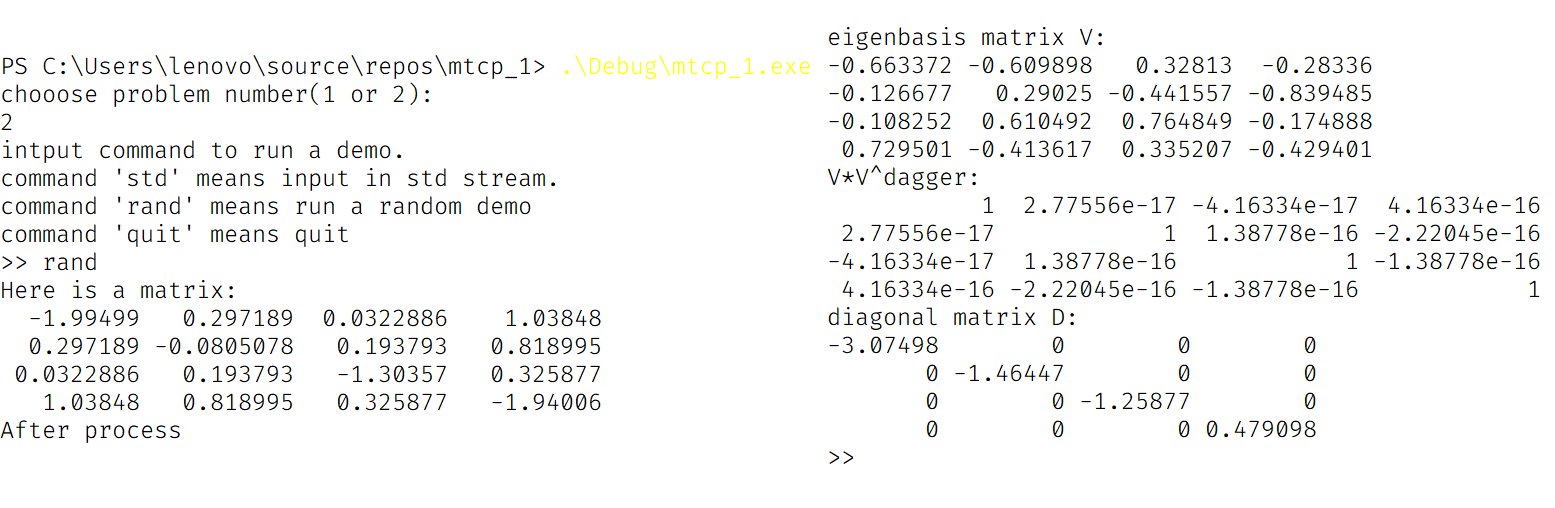
\includegraphics[width = 1.7\textheight]{img/result2.png}
        \caption{demo: input from random symetric matrix}
    \end{figure}
\end{frame}
